\chapter{Linear Models and Representation}
\label{ch:linear-models}

Can one weighted sum already solve the task? It is a serious question. Once a representation has been chosen, the simplest model that takes those features and predicts a label is a linear one---one coefficient per feature, summed, optionally squashed. If that model already performs well, every later complication has to justify itself against it. If it fails, the failure pattern usually says exactly what kind of complication is needed: branches, margins, neighborhoods, latent structure, or a learned representation.

This chapter treats linear models not as old formulas to memorize but as a disciplined test of representation. A strong representation and a controlled linear baseline often go further than beginners expect, and when they fail, the failure pattern is usually informative. The chapter moves from feature maps to the generic weighted-sum pipeline, then to linear regression, logistic regression, coefficient reading, and regularization. Its concrete deliverable is a first baseline design sheet stating what the model sees, what it predicts, how its coefficients may be read safely, how it will be regularized, and what specific failure would justify leaving linearity.

\section{Opening Dilemma: Is One Weighted Sum Enough?}

Suppose we have already framed an early student-support task, chosen an evaluation plan, and agreed on what counts as a useful prediction. A support team wants to use early quizzes, submissions, and platform activity to flag students who may need timely human outreach. We still need a first model family. A deep model may eventually win, but it is rarely the right first move. The right first move is usually the simplest serious model that can show whether the representation already contains most of the signal.

That is why linear models appear early in this book. They are not here because they are old or mathematically easy. They are here because they make the route from representation to prediction unusually visible. A linear model says: encode the example as numbers, attach a weight to each one, add the contributions, and transform the result if needed. This simplicity is pedagogically valuable because it makes failure diagnostic instead of mysterious.

Keep the early student-support setting in view through this chapter. Later chapters widen the institutional workflow into message routing, retrieval, and grounded answers, but the first baseline question is simpler: can a transparent weighted-sum model already surface the right cases for human review? Each major section turns that one question into a modeling discipline---choose the representation, understand the score, read the coefficients carefully, control complexity, and diagnose failure structurally.

CDC guidance for Youth Risk Behavior Survey trend analysis still uses logistic regression for dichotomous risk behaviors and linear regression for continuous ones \citep{cdc_yrbs_trends}. These models are not teaching artifacts. They remain standard analytical tools in serious public-health workflows.

\begin{table}[t]
\centering
\small
\setlength{\tabcolsep}{4pt}
\begin{tabular}{p{3.41cm}p{6.82cm}}
\toprule
Problem shape & What linear models are usually good for \\
\midrule
Structured tabular data & Fast baselines, interpretable coefficients, and surprisingly strong performance when the feature design is careful \\
Sparse text features & Reliable bag-of-words or term frequency--inverse document frequency (TF--IDF) baselines where weighted word evidence already carries most of the signal \\
High-dimensional raw images, audio, or long sequences & Usually only baseline value unless a strong representation has already been learned elsewhere \\
\bottomrule
\end{tabular}
\caption{Linear models are not universal, but they are often the right first serious baseline for structured and sparse problems.}
\label{tab:linear-model-regimes}
\end{table}

\section{Representation Is the Model}

The heart of this chapter is not a fitting rule. It is a representation question.

\begin{definition}[Feature]
A feature is a measurable attribute used to represent an example for a model. Features may be numeric, binary, categorical after encoding, counts, ratios, embeddings, or other derived quantities.
\end{definition}

This definition sounds technical, but its consequences are conceptual. A feature is not just a column in a table; it is a modeling decision. Choosing floor area, age, and distance to transit as features for house-price prediction asserts that these properties may help explain price. Encoding words or character patterns for spam detection asserts that certain language or formatting patterns may carry useful signal. Feature design is not bookkeeping after the interesting part---it is where much of the interesting part already happens.

That is why representation is already part of the model. The model does not see ``a house in a good neighborhood'' or ``a student who is disengaging.'' It sees the encoded representation. Someone must decide which numbers or indicators could plausibly carry the relevant information.

\textbf{Representation audit.} Before fitting a model, ask:
\begin{itemize}[leftmargin=*]
\item What is the raw input?
\item What is the encoded representation?
\item What information is lost by the encoding?
\item What assumptions are being inserted artificially?
\end{itemize}

\subsection{Raw Inputs and Feature Maps}

Sometimes the raw input is already numeric and usable. Age, temperature, income, and elapsed time fit that description. Often, though, raw inputs must be transformed before a linear model can use them effectively. Text must become counts, indicator variables, or embeddings. Categories must be encoded. Dates may need to become cyclic or calendar-aware features. Interactions may need to be added explicitly when they matter.

We often write this as a feature map $\phi(x)$, a compact way to say ``the encoded version of the raw example $x$ that the model actually sees'':
\[
\phi(x) = [\phi_1(x), \phi_2(x), \ldots, \phi_d(x)]^\top.
\]
The model operates on $\phi(x)$ rather than on the raw input. This notation separates two sources of modeling power: the \emph{representation} chosen by the feature map and the \emph{fitted weights} learned by the model.

A weak representation cannot be saved by better weights. A strong representation can make even a simple weighted sum work well.

The linear-model workflow is compact: encode the raw input, fit a baseline, inspect residuals or errors, then ask whether the representation needs interaction terms, scaling, or a different feature map before changing model family.

If the notation $\phi(x)$ is new, read it as ``the version of the raw input that the model actually uses.'' In practice, this is where most of the modeling judgment lives.

From here on, the notation is compressed: unless the distinction matters, \(x\) means the \emph{encoded feature vector} rather than the raw object. When the distinction matters, think in two layers:
\[
x_{\text{raw}} \longrightarrow \phi(x_{\text{raw}}) \longrightarrow w^\top \phi(x_{\text{raw}}) + b.
\]
That small discipline prevents a common beginner confusion. The coefficients do not multiply ``the email'' or ``the apartment'' in the abstract. They multiply the engineered features the model was given.

\begin{example}[From Raw Input to Feature Vector]
Suppose the raw email is ``FREE cash offer today,'' sent from an unfamiliar domain and containing two links. A simple feature map might turn this raw message into
\[
\phi(x_{\text{raw}}) =
\begin{bmatrix}
1 \\
2 \\
0.8 \\
0
\end{bmatrix},
\]
where the four entries are an urgent-language indicator, the number of links, a sender-risk score, and whether the sender matches a trusted course domain. The linear model never sees the sentence directly---only these four numbers. If the feature map throws away evidence that later turns out to matter, the weighted sum cannot reconstruct it.
\end{example}

\subsection{Interaction Features and Basis Expansion}

A linear model on raw features can only express additive effects: each feature's contribution is independent of every other. But many real problems have inherently interactive structure. Floor area's effect on apartment price may depend on the neighborhood. Missed assignments may matter more in the last week of term than in the first.

\emph{Interaction features} make these joint effects explicit. An interaction term for two features $x_1$ and $x_2$ is their product $x_1 x_2$. Once that product is added as a new coordinate, the linear model can assign a separate coefficient to the joint effect.

\emph{Basis expansion} generalizes the idea. Any function of the raw inputs can be added as a new feature: squares, square roots, logarithms, threshold indicators, products of three or more features, or Fourier-style sinusoidal terms. The resulting feature map $\phi(x)$ may be much richer than the original input, but the model on top of it remains linear in the expanded features.

\begin{example}[Interaction Features in Practice]
Suppose we predict student risk from two features: fraction of assignments missed ($x_1$) and week of semester ($x_2$). On their own, missing a moderate fraction of assignments may be less alarming in week two than in week ten. Adding the product $x_1 x_2$ lets the model express that the effect of missed assignments grows with time. The coefficient on $x_1 x_2$ is positive if late-semester missing work is especially predictive, regardless of what the individual coefficients on $x_1$ and $x_2$ say.
\end{example}

If the feature map is $\phi(x) = [x_1,\, x_2,\, x_1^2,\, x_2^2,\, x_1 x_2]^\top$, then the model $w^\top \phi(x) + b$ is nonlinear in the raw input $x$ but still linear in the expanded coordinates $\phi(x)$. Training with gradient descent or ordinary least squares still applies without modification. The representational power comes from the engineer's choice of $\phi$, not from a more complex model family.

Why does this matter? Many students conclude too quickly that linear models are only useful for obviously linear worlds. Basis expansion shows that a thoughtful feature map can extend a linear model's expressiveness considerably. The cost is interpretability: once features interact, individual coefficients are harder to read as standalone effects. The judgment call is whether the gain in fit justifies the loss in narrative clarity.

Add interaction features deliberately, not exhaustively. All pairwise products of $d$ features produce $d(d-1)/2$ new coordinates. On a dataset with hundreds of features, that explosion causes severe overfitting and slow training. Add interactions when domain knowledge suggests a specific joint effect, and test whether each addition improves held-out performance.

\subsection{Common Feature Types}

Numeric features are the simplest case. For house-price prediction, a feature like floor area can enter directly as a number. Even then, choices remain. Total area or its logarithm? Centered and scaled, or raw? An interaction between area and neighborhood, or not?

Categorical features require more care. A feature like neighborhood, major, product category, or browser type cannot be inserted as a single integer without creating an artificial ordering. The common solution is one-hot encoding: each category gets its own indicator variable. With an explicit intercept, practitioners usually drop one indicator as the reference category or use regularization carefully to avoid perfect collinearity.

Text features are often sparse. A bag-of-words representation includes one feature per word, recording whether the word appears or how often. This is one reason linear models remain strong in text classification: even when the representation is high-dimensional, the modeling assumption is still a weighted combination of informative signals.

\begin{figure}[t]
\centering
\definecolor{c3blue}{RGB}{56,103,170}
\definecolor{c3blueBg}{RGB}{220,233,251}
\definecolor{c3headBg}{RGB}{235,242,253}
\resizebox{\linewidth}{!}{%
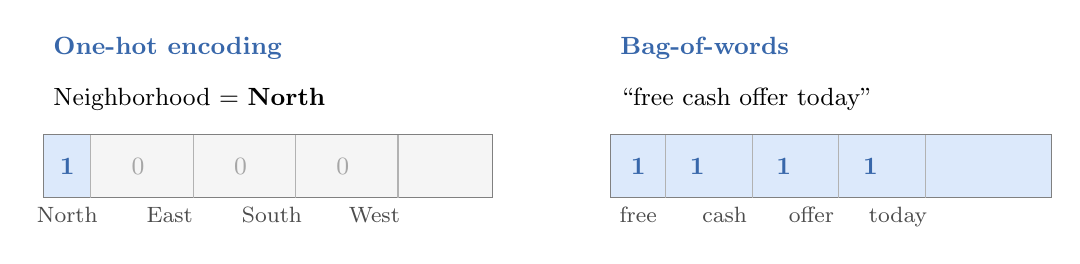
\begin{tikzpicture}[font=\small]
%% ---- One-hot encoding ----
\begin{scope}
  \node[anchor=west, font=\small\bfseries, color=c3blue] at (0,3.0) {One-hot encoding};
  \node[anchor=west] at (0,2.35) {Neighborhood = \textbf{North}};
  \fill[gray!8]   (0,1.1)   rectangle (5.7,1.9);
  \fill[c3blueBg] (0,1.1)   rectangle (0.6,1.9);
  \draw[black!50] (0,1.1)   rectangle (5.7,1.9);
  \foreach \x in {0.6,1.9,3.2,4.5}
    \draw[black!30] (\x,1.1) -- (\x,1.9);
  \foreach \x/\lbl in {0.6/North,1.9/East,3.2/South,4.5/West}
    \node[below, font=\footnotesize, black!70] at (\x-0.3,1.1) {\lbl};
  \node[font=\small\bfseries, color=c3blue] at (0.3,1.5) {1};
  \node[font=\small, black!35] at (1.2,1.5) {0};
  \node[font=\small, black!35] at (2.5,1.5) {0};
  \node[font=\small, black!35] at (3.8,1.5) {0};
\end{scope}
%% ---- Bag-of-words ----
\begin{scope}[xshift=7.2cm]
  \node[anchor=west, font=\small\bfseries, color=c3blue] at (0,3.0) {Bag-of-words};
  \node[anchor=west] at (0,2.35) {``free cash offer today''};
  \fill[c3blueBg] (0,1.1) rectangle (5.6,1.9);
  \draw[black!50] (0,1.1) rectangle (5.6,1.9);
  \foreach \x/\lbl in {0.7/free,1.8/cash,2.9/offer,4.0/today}
  {
    \draw[black!30] (\x,1.1) -- (\x,1.9);
    \node[below, font=\footnotesize, black!70] at (\x-0.35,1.1) {\lbl};
  }
  \node[font=\small\bfseries, color=c3blue] at (0.35,1.5) {1};
  \node[font=\small\bfseries, color=c3blue] at (1.1,1.5)  {1};
  \node[font=\small\bfseries, color=c3blue] at (2.2,1.5)  {1};
  \node[font=\small\bfseries, color=c3blue] at (3.3,1.5)  {1};
\end{scope}
\end{tikzpicture}%
}
\caption{Representation choices make assumptions visible. One-hot vectors avoid fake category ordering, while bag-of-words vectors make text usable through sparse counts.}
\label{fig:feature-encodings}
\end{figure}

\begin{example}[Feature Design for Housing]
Suppose we want to predict apartment prices. Raw inputs might include address, floor area, year built, floor number, and text descriptions. A reasonable first feature set could contain area, number of bedrooms, age, distance to the city center, and one-hot neighborhood indicators. This set already makes several claims: location matters, age matters, and neighborhood effects deserve separate coefficients rather than a single numeric code.
\end{example}

\begin{example}[Feature Design Across Public Tasks]
The same logic recurs across public tasks. A sports-shot prediction problem invites structured tabular features such as player position, shot distance, and remaining time. A news topic classification problem invites sparse lexical features or TF--IDF vectors. The tasks differ, but the chapter's question is the same: what representation would let a weighted sum detect the relevant signal?
\end{example}

\section{The Generic Linear Pipeline}

Before splitting into regression and classification, it helps to establish the pipeline they share.

\begin{figure}[t]
\centering
\definecolor{c3pipeA}{RGB}{220,233,251}
\definecolor{c3pipeB}{RGB}{210,238,220}
\definecolor{c3pipeC}{RGB}{254,242,214}
\definecolor{c3pipeD}{RGB}{237,224,250}
\definecolor{c3pipeLineA}{RGB}{56,103,170}
\definecolor{c3pipeLineB}{RGB}{26,112,64}
\definecolor{c3pipeLineC}{RGB}{184,92,16}
\definecolor{c3pipeLineD}{RGB}{100,50,160}
\resizebox{\linewidth}{!}{%
\begin{tikzpicture}[
  boxA/.style={draw=c3pipeLineA, rounded corners, align=center, minimum height=1.0cm, minimum width=2.05cm, fill=c3pipeA, text=c3pipeLineA, font=\small\bfseries},
  boxB/.style={draw=c3pipeLineB, rounded corners, align=center, minimum height=1.0cm, minimum width=2.05cm, fill=c3pipeB, text=c3pipeLineB, font=\small\bfseries},
  boxC/.style={draw=c3pipeLineA, rounded corners, align=center, minimum height=1.0cm, minimum width=2.05cm, fill=c3pipeA, text=c3pipeLineA, font=\small\bfseries},
  boxD/.style={draw=c3pipeLineC, rounded corners, align=center, minimum height=1.0cm, minimum width=2.05cm, fill=c3pipeC, text=c3pipeLineC, font=\small\bfseries},
  boxE/.style={draw=c3pipeLineD, rounded corners, align=center, minimum height=1.0cm, minimum width=2.05cm, fill=c3pipeD, text=c3pipeLineD, font=\small\bfseries},
  arrow/.style={-Latex, thick, black!60}
]
\node[boxA] (raw)      {Raw input};
\node[boxB, right=0.6cm of raw]    (phi)      {Feature map\\$\phi(x)$};
\node[boxC, right=0.6cm of phi]    (score)    {Weighted sum\\$w^\top \phi(x) + b$};
\node[boxD, right=0.6cm of score]  (transform){Output transform};
\node[boxE, right=0.6cm of transform](decision){Decision use};
\draw[arrow] (raw)       -- (phi);
\draw[arrow] (phi)       -- (score);
\draw[arrow] (score)     -- (transform);
\draw[arrow] (transform) -- (decision);
\end{tikzpicture}%
}
\caption{Linear-model pipeline.}
\label{fig:linear-model-pipeline}
\end{figure}

\begin{codeexample}[caption={A generic feature pipeline for a linear model}]
raw_example = collect_input()
features = feature_map(raw_example)
score = dot(weights, features) + bias
prediction = output_transform(score)
\end{codeexample}

This small program is worth remembering. Linear regression and logistic regression are two instances of this general pattern. The only real difference is what the output transform does. The score-producing core stays the same, which is why the chapter can teach both models as one pipeline rather than as two unrelated formulas.

\textbf{Structural rescue test.} If a linear baseline fails, ask two questions in order:
\begin{itemize}[leftmargin=*]
\item Could one additional transformed feature make the missing pattern visible, such as area-squared or attendance times homework score?
\item If not, what kind of structure is missing entirely: local neighborhoods, branching rules, sequence order, or a learned representation?
\end{itemize}
Do not jump from ``the line failed'' to ``the whole model family failed.'' First test whether the representation, not the weighted sum, is the real bottleneck.

\begin{decisionbox}
\textbf{Which linear family first?}
\begin{itemize}[leftmargin=*]
\item Numeric target such as price, time, or demand: start with linear regression.
\item Binary target or event probability such as spam versus not spam: start with logistic regression.
\item Need multiclass probabilities: the same score-then-transform logic extends, but the chapter's conceptual split remains numeric output versus probability output.
\item Need an action rather than only a score: keep the fitted score, the probability, and the thresholding rule conceptually separate.
\end{itemize}
\end{decisionbox}

\section{Linear Regression as the First Concrete Case}

\begin{definition}[Linear Regression]
Linear regression predicts a numeric target as an affine function of the features, meaning a weighted sum plus an intercept:
\[
\hat{y} = w^\top x + b,
\]
where $x$ is the feature vector, $w$ is the vector of coefficients, and $b$ is the intercept.
\end{definition}

Here again, \(x\) means the representation after encoding. If the notation feels too compressed, mentally expand the model to \(\hat{y} = w^\top \phi(x_{\text{raw}}) + b\). That expansion is the cleaner reminder that linear modeling and feature design are one pipeline, not two disconnected steps.

The word \emph{linear} refers to linearity in the parameters and the feature representation, not in the raw input. The distinction matters. A linear model can still express nonlinear behavior in the original input when the features themselves encode nonlinear transformations.

\subsection{Residuals and Squared Error}

For a training example $(x_i, y_i)$, the prediction error is the residual:
\[
r_i = y_i - \hat{y}_i.
\]
Linear regression is usually fit by minimizing the mean squared residual:
\[
\text{MSE} = \frac{1}{n} \sum_{i=1}^{n} (y_i - \hat{y}_i)^2.
\]

Chapter 2 explained why squared error is a useful training loss. Here the important skill is more concrete: move comfortably from feature values to prediction to residual, and read what the residual says about the baseline. A positive residual means the model predicted too low; a negative residual means it predicted too high.

The theorem below explains why least squares is geometrically special. Skip it on a first read until after the apartment-price example. The core skill is reading residuals and diagnosing what a linear baseline can and cannot express.

\begin{theorem}[Least-squares residuals are orthogonal to the fitted space]
In ordinary least squares, let \(X\) be the design matrix augmented with an intercept column, so the affine model \(w^\top x+b\) can be written as a single matrix product \(X w\) (with \(w\) likewise extended by the intercept term). If \(\hat{y}=X\hat{w}\) is the fitted value vector and \(r=y-\hat{y}\) is the residual vector, then
\[
X^\top r = 0.
\]
Equivalently, the residual vector is orthogonal to every column of the design matrix and therefore to every direction the linear model was allowed to use.
\end{theorem}

\begin{proof}
Ordinary least squares minimizes \(\|y-Xw\|_2^2\). Differentiating with respect to \(w\) and setting the derivative to zero gives the normal equations
\[
X^\top (y-X\hat{w}) = 0.
\]
Since \(r=y-X\hat{w}\), this is exactly \(X^\top r=0\).
\end{proof}

This is the geometric meaning of best fit in a linear model: once the data has been projected onto the allowed feature space, the leftover error cannot be reduced by moving further inside that same space.

\subsection{Minimizing the Loss: Gradient Descent}

Ordinary least squares has a closed-form solution, but gradient descent is the reusable optimization procedure that matters throughout the book. Starting from some initial weight vector $w$, we repeatedly move the weights in the direction that decreases the loss fastest. The gradient $\nabla_w \mathcal{L}$ points uphill, so we subtract a small multiple of it:
\[
w \leftarrow w - \eta \, \nabla_w \mathcal{L}(w),
\]
where $\eta > 0$ is the learning rate, controlling step size. For MSE, the gradient with respect to weight $w_j$ is
\[
\frac{\partial \,\text{MSE}}{\partial w_j} = \frac{2}{n} \sum_{i=1}^{n} (\hat{y}_i - y_i) \, x_{ij}.
\]
Each gradient component tells one weight which direction to move and by how much. One application of this update is one gradient descent step.

\begin{codeexample}[caption={From scratch: one gradient descent step for linear regression}]
# Student support task: features are (attendance_rate, late_submission_rate),
# target is risk_score (higher means more at-risk)
data = [
    ([0.9, 0.1], 0.2),   # high attendance, few lates -> low risk
    ([0.7, 0.3], 0.4),
    ([0.5, 0.5], 0.6),
    ([0.3, 0.7], 0.7),
    ([0.2, 0.8], 0.9),   # low attendance, many lates -> high risk
]

learning_rate = 0.1
weights = [0.0, 0.0]   # one weight per feature; no explicit bias here
n = len(data)

def dot(a, b):
    return sum(wi * xi for wi, xi in zip(a, b))

# --- compute MSE loss before the step ---
loss_before = sum((dot(weights, x) - y) ** 2 for x, y in data) / n

# --- compute gradient ---
gradient = [0.0] * len(weights)
for x, y in data:
    error = dot(weights, x) - y     # (pred - true)
    for j in range(len(weights)):
        gradient[j] += (2 / n) * error * x[j]

# --- update weights ---
weights = [weights[j] - learning_rate * gradient[j]
           for j in range(len(weights))]

# --- compute MSE loss after the step ---
loss_after = sum((dot(weights, x) - y) ** 2 for x, y in data) / n

print(round(loss_before, 4))   # loss before the step
print(round(loss_after, 4))    # loss after one correction
\end{codeexample}

Running this program produces a smaller loss after a single step. The point is to show the mechanics of gradient descent, not to settle each feature's final semantic role from one update. Because the model begins near zero and the features are not centered, the earliest steps mainly reflect the model's effort to move away from systematic underprediction. In a fitted model with an explicit bias term and centered or standardized inputs, the eventual sign and magnitude of each coefficient become easier to interpret.

\begin{sanitycheck}
\textbf{Loss should strictly decrease after one gradient step.} For a convex loss and a small enough learning rate, $\mathcal{L}(w - \eta \nabla \mathcal{L}(w)) < \mathcal{L}(w)$. After the first step in any from-scratch implementation, print both losses and verify the inequality. If \verb|loss_after >= loss_before|, the learning rate is too large for the current curvature (halve it and try again), the gradient is computed incorrectly (run the finite-difference check from Mathematical Bridge~II), or the loss surface is non-convex in a region with a poor initialization. ``Loss did not go down on the first step'' should never be brushed past as bad luck; it is a small-cost-to-catch, large-cost-to-miss bug.
\end{sanitycheck}

\begin{figure}[t]
\centering
\definecolor{c3fitLine}{RGB}{56,103,170}
\definecolor{c3residLine}{RGB}{180,40,40}
\resizebox{\linewidth}{!}{%
\begin{tikzpicture}[x=1cm,y=1.4cm,font=\small]
  \draw[->,thick,black!70] (-0.2,0) -- (8.8,0) node[right] {area};
  \draw[->,thick,black!70] (0,-0.2) -- (0,6.2) node[above] {price};
  %% Fitted line
  \draw[c3fitLine,thick] (0.3,0.41) -- (8.5,4.92);
  %% Residuals (dashed red lines between fitted line and data point)
  \draw[dashed,c3residLine,line width=0.9pt] (1.2,0.86) -- (1.2,0.90);
  \draw[dashed,c3residLine,line width=0.9pt] (2.0,1.35) -- (2.0,1.47);
  \draw[dashed,c3residLine,line width=0.9pt] (4.2,2.56) -- (4.2,2.85);
  \draw[dashed,c3residLine,line width=0.9pt] (5.6,3.33) -- (5.6,3.53);
  \draw[dashed,c3residLine,line width=0.9pt] (7.2,4.21) -- (7.2,4.91);
  %% Data points
  \foreach \px/\py in {1.2/0.86,2.0/1.47,3.0/1.90,4.2/2.85,5.6/3.53,7.2/4.91}
    \filldraw[c3fitLine,fill=c3fitLine!80] (\px,\py) circle (3pt);
  %% Labels — fitted line label below the line in open space
  \node[rotate=29, anchor=north, font=\footnotesize, c3fitLine] at (2.2,1.25) {fitted line};
  %% Residuals label — below the chart, right side, with short upward leader to mid residual
  \node[anchor=north west, font=\footnotesize, align=left, text width=2.8cm] at (6.5,2.0)
      {\textcolor{c3residLine}{residuals:} vertical prediction errors};
  %% leader: straight right from residual at x=4.2, then straight down
  \draw[<-,thin,c3residLine] (4.2,2.56) -- (6.4,2.56) -- (6.4,2.0);
\end{tikzpicture}%
}
\caption{Linear regression predicts with a line in feature space. Residuals measure how far the observed targets fall above or below the fitted prediction.}
\label{fig:regression-residuals}
\end{figure}

\subsection{Worked Example: Predicting Apartment Prices}

Imagine a small apartment dataset with features for floor area, number of bedrooms, and age of the building.

\begin{table}[t]
\centering
\begin{tabular}{>{\centering}p{1.6cm}>{\centering}p{1.7cm}>{\centering}p{1.5cm}>{\centering}p{1.7cm}>{\centering\arraybackslash}p{2.2cm}}
\toprule
Apt & Area ($m^2$) & Beds & Age (yr) & Price (k) \\
\midrule
A & 50 & 1 & 25 & 175 \\
B & 60 & 2 & 18 & 220 \\
C & 70 & 2 & 12 & 260 \\
D & 80 & 3 & 8 & 310 \\
E & 90 & 3 & 5 & 350 \\
F & 105 & 4 & 3 & 405 \\
\bottomrule
\end{tabular}
\caption{A tiny housing table is enough to make the regression story concrete.}
\label{tab:apartment-example}
\end{table}

A fitted model might look like
\[
\hat{y} = 48 + 3.1 \cdot \text{area} + 11 \cdot \text{bedrooms} - 1.4 \cdot \text{age},
\]
where the target is measured in thousands of currency units. The model says that, all else equal, each additional square meter adds about 3.1 thousand to the predicted price, each extra bedroom adds 11 thousand, and each additional year of age subtracts about 1.4 thousand.

Now take an apartment with 82 square meters, 3 bedrooms, and age 6:
\[
\hat{y} = 48 + 3.1(82) + 11(3) - 1.4(6) = 326.8.
\]
If the actual sale price turned out to be 338, the residual would be
\[
r = 338 - 326.8 = 11.2.
\]

That is the first concrete skill this chapter wants to automate: move from encoded features to a predicted numeric value, then inspect the residual rather than interpreting the formula in isolation.

\begin{warningbox}
An interpretable model is not the same as a correct interpretation. Coefficients are interpretable only relative to the features included, their scales, and the correlations among them.
\end{warningbox}

\subsection{Residual Diagnostics}

Residuals are not bookkeeping after the fit. If residuals curve with the fitted values, the representation is probably missing nonlinear structure. If their spread grows with the prediction, the error variance is not constant. If one slice produces extreme residuals, that slice may need a separate feature, a missingness indicator, or a different interaction term. In a linear baseline, residual plots are often the fastest way to learn what structure the representation left out.

\begin{table}[t]
\centering
\small
\setlength{\tabcolsep}{4pt}
\begin{tabular}{p{3.0cm}p{3.25cm}p{3.55cm}}
\toprule
Residual pattern & Likely missing structure & Next baseline move \\
\midrule
Residuals curve with fitted value & nonlinear relationship in the raw feature & add a squared, log, or spline-like feature and validate it \\
Residual spread grows with prediction & error variance changes by scale & try a transformed target or report scale-aware uncertainty \\
One operational slice has extreme residuals & missing slice-specific signal or shifted data source & add a slice indicator, missingness flag, or separate slice evaluation \\
\bottomrule
\end{tabular}
\caption{Residual diagnostics are useful only when they lead to a concrete next baseline move rather than a vague sense that the model is weak.}
\label{tab:residual-diagnostic-next-move}
\end{table}

\subsection{Linear in the Parameters, Not Necessarily in the World}

Students often hear ``linear model'' and imagine ``straight line in reality.'' That picture is too narrow. The model is linear in the \emph{parameters and representation}, not necessarily in the raw input.

\begin{figure}[t]
\centering
\definecolor{c3linBlue}{RGB}{56,103,170}
\definecolor{c3ptGray}{RGB}{60,60,60}
\resizebox{\linewidth}{!}{%
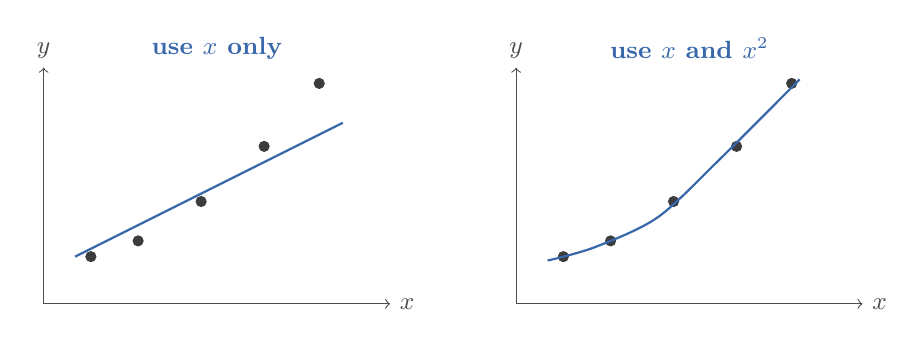
\begin{tikzpicture}[font=\small]
%% Panel A: use x only → straight line
\begin{scope}
  \draw[->,black!70] (0,0) -- (4.4,0) node[right] {$x$};
  \draw[->,black!70] (0,0) -- (0,3.0) node[above] {$y$};
  \foreach \px/\py in {0.6/0.6,1.2/0.8,2.0/1.3,2.8/2.0,3.5/2.8}
    \filldraw[c3ptGray] (\px,\py) circle (1.8pt);
  \draw[c3linBlue,thick] (0.4,0.6) -- (3.8,2.3);
  \node[c3linBlue, font=\small\bfseries] at (2.2,3.25) {use $x$ only};
\end{scope}
%% Panel B: use x and x^2 → curved fit
\begin{scope}[xshift=6.0cm]
  \draw[->,black!70] (0,0) -- (4.4,0) node[right] {$x$};
  \draw[->,black!70] (0,0) -- (0,3.0) node[above] {$y$};
  \foreach \px/\py in {0.6/0.6,1.2/0.8,2.0/1.3,2.8/2.0,3.5/2.8}
    \filldraw[c3ptGray] (\px,\py) circle (1.8pt);
  \draw[c3linBlue,thick] plot[smooth] coordinates {(0.4,0.55)(1.0,0.72)(1.8,1.1)(2.6,1.85)(3.6,2.85)};
  \node[c3linBlue, font=\small\bfseries] at (2.2,3.25) {use $x$ and $x^2$};
\end{scope}
\end{tikzpicture}%
}
\caption{Both panels can come from linear models. The right panel is still linear in the parameters because the nonlinear behavior is carried by the feature map, not by a nonlinear weighting rule.}
\label{fig:linear-in-parameters}
\end{figure}

Suppose Model A uses only area. Model B uses both area and area-squared. Model B can represent curvature in the relationship between area and price even while staying linear in the parameters. That is one of the chapter's highest-value lessons: ``linear model'' names the weighting rule, not the shape of the world.

With the shared score-producing pipeline in place, the next distinction is the output type---first a numeric target, then a probability target.

\section{Logistic Regression as Score-to-Probability Modeling}

Linear regression predicts unrestricted numeric outputs, which makes it unsuitable for binary classification. When the target is whether an email is spam or whether a student needs support, we want a probability or a class label, not an arbitrary real number such as $1.7$ or $-0.8$.

Logistic regression keeps the weighted-sum backbone and changes only the output transform. The model first computes a raw score, often called the \emph{logit},
\[
z = w^\top x + b,
\]
and then maps that score to a probability through the sigmoid function:
\begin{align*}
\sigma(z) &= \frac{1}{1 + e^{-z}}, \\
P(y=1 \mid x) &= \sigma(w^\top x + b).
\end{align*}

In predictive language, this is the model's estimated conditional probability, not automatically a calibrated real-world frequency. The generic pipeline matters here. Linear regression uses the identity transform. Logistic regression uses the sigmoid. The change is not cosmetic: logistic regression is trained against a classification objective such as log loss, and its output is meant to support probability estimation and threshold policy rather than unrestricted numeric prediction. Keep three layers separate throughout: score, probability, and decision rule.

Logistic regression has a linear score and a linear decision boundary in the encoded feature space, but the final probability is nonlinear in the score.

\subsection{From Score to Probability}

Why the sigmoid? It maps any real-valued score into the interval $(0,1)$, so the output can be read as a probability, and it preserves ordering: larger scores correspond to larger predicted probabilities.

Another useful viewpoint is through the log-odds:
\[
\log \frac{P(y=1 \mid x)}{1 - P(y=1 \mid x)} = w^\top x + b.
\]
This follows directly from the sigmoid. If $p=\sigma(z)=\frac{1}{1+e^{-z}}$, then $1-p=\frac{e^{-z}}{1+e^{-z}}$, so
\[
\frac{p}{1-p}=e^z
\quad\Longrightarrow\quad
\log\frac{p}{1-p}=z=w^\top x+b.
\]
Students need not memorize this form, but it clarifies why logistic regression is mathematically clean: the classification problem is still built from a linear scoring rule.

\begin{figure}[t]
\centering
\definecolor{c3sigBlue}{RGB}{56,103,170}
\definecolor{c3sigAmber}{RGB}{184,92,16}
\resizebox{\linewidth}{!}{%
\begin{tikzpicture}[x=1.4cm,y=3.2cm,font=\small]
  \draw[->,black!70] (-3.0,0) -- (3.2,0) node[right] {logit $z$};
  \draw[->,black!70] (0,-0.02) -- (0,1.08) node[above] {probability};
  %% Sigmoid curve
  \draw[c3sigBlue,thick,domain=-2.8:2.8,samples=100,smooth] plot (\x,{1/(1+exp(-\x))});
  %% Reference dashed lines
  \draw[c3sigAmber,dashed,thin] (-2,0) -- (-2,{1/(1+exp(2))});
  \draw[c3sigAmber,dashed,thin] (2,0)  -- (2,{1/(1+exp(-2))});
  \draw[c3sigAmber,dashed,thin] (0,0)  -- (0,0.5);
  %% Tick labels
  \foreach \z/\lbl in {-2/$-2$,0/$0$,2/$2$}
    \node[below, font=\footnotesize, black!70] at (\z,0) {\lbl};
  \node[left, font=\footnotesize, black!70] at (0,0.12) {$0.12$};
  \node[left, font=\footnotesize, black!70] at (0,0.5)  {$0.50$};
  \node[left, font=\footnotesize, black!70] at (0,0.88) {$0.88$};
\end{tikzpicture}%
}
\caption{Logistic regression turns a linear score into a probability. The key distinction is score $\rightarrow$ probability $\rightarrow$ thresholded decision. Those are three different objects.}
\label{fig:sigmoid-curve}
\end{figure}

\begin{warningbox}
Probability and odds are not the same. A probability of $0.8$ means ``80\% chance.'' Odds of $4{:}1$ mean four positive cases for every one negative case. Logistic regression becomes easier to interpret once that distinction is kept explicit.
\end{warningbox}

A one-unit increase in feature $x_j$ changes the log-odds by $w_j$ and multiplies the odds by $e^{w_j}$, holding the other encoded features fixed. That is often the cleanest coefficient interpretation in logistic regression.

\begin{theorem}[A $0.5$ logistic threshold is a score threshold]
If logistic regression predicts the positive class whenever $P(y=1 \mid x) \ge 0.5$, then this rule is exactly the same as predicting the positive class whenever
\[
w^\top x + b \ge 0.
\]
The boundary between the two decisions is therefore the set of inputs for which
\[
w^\top x + b = 0.
\]
\end{theorem}

\begin{proof}
Let $z = w^\top x + b$. The sigmoid sends $z=0$ to $\sigma(0)=0.5$, and larger scores produce larger probabilities. Therefore
\[
P(y=1 \mid x) \ge 0.5
\quad \Longleftrightarrow \quad
\sigma(z) \ge 0.5
\quad \Longleftrightarrow \quad
z \ge 0.
\]
Substituting back gives the result.
\end{proof}

For any probability threshold $\tau \in (0,1)$, the equivalent score cutoff is
\[
w^\top x + b \ge \log\frac{\tau}{1-\tau}.
\]
The theorem's $0.5$ case is the special case where this cutoff is zero.

\subsection{Worked Example: A Spam Probability}

Suppose a mail system wants to estimate the probability that a message is spam. Features might include a suspicious-link signal, an urgent-language signal, and a sender-risk score. A logistic model can learn that stronger values on these features push the score upward.

To see the mechanics directly, suppose the feature vector for one message is
\[
x =
\begin{bmatrix}
0.6 \\
0.8 \\
0.4
\end{bmatrix},
\]
where the three components represent scaled signals for suspicious links, urgent sales language, and sender-risk score. Let the fitted logistic-regression parameters be
\[
w =
\begin{bmatrix}
1.4 \\
1.8 \\
1.1
\end{bmatrix},
\qquad
b=-2.0.
\]
The linear score is therefore
\[
z = w^\top x + b = 1.4(0.6) + 1.8(0.8) + 1.1(0.4) - 2.0 = 0.72.
\]
Applying the sigmoid gives
\[
P(y=1 \mid x) = \sigma(0.72) \approx 0.673.
\]

\begin{codeexample}[caption={Algorithm sketch: logistic score and probability}]
Input: feature vector x, weight vector w, bias b
score = dot(w, x) + b
probability = 1 / (1 + exp(-score))
if probability >= 0.5:
    label = 1
else:
    label = 0
return score, probability, label
\end{codeexample}

This tiny program mirrors the worked example exactly, and it is worth typing once. The purpose is not software engineering. The purpose is to make the pipeline concrete enough that a student can move from feature values to score to probability to label without hiding behind a library call.

Here ``all else equal'' means holding the encoded features fixed inside the fitted model, not holding the whole world fixed.

\begin{table}[t]
\centering
\setlength{\tabcolsep}{4pt}
\begin{tabular}{>{\raggedright}p{3.0cm}>{\centering}p{1.1cm}>{\centering}p{2.2cm}>{\centering\arraybackslash}p{3.1cm}}
\toprule
Feature & Value & Coefficient & Contribution to $z$ \\
\midrule
Suspicious-link signal & 0.6 & 1.4 & 0.84 \\
Urgent-language signal & 0.8 & 1.8 & 1.44 \\
Sender-risk score & 0.4 & 1.1 & 0.44 \\
Bias & --- & --- & $-2.00$ \\
\midrule
Total logit & --- & --- & 0.72 \\
\bottomrule
\end{tabular}
\caption{A by-hand logistic-regression score decomposition.}
\label{tab:logistic-decomposition}
\end{table}

At a spam threshold of $0.5$ the message is flagged; at $0.7$ it is not. Chapter 2 covered threshold policy in detail. Here the example serves a narrower purpose: keep the boundary clear between the model's score and probability and the larger system's decision about how to act.

\begin{table}[t]
\centering
\small
\setlength{\tabcolsep}{6pt}
\begin{tabular}{ccc}
\toprule
Logit $z$ & Probability $\sigma(z)$ & If threshold is $0.5$ \\
\midrule
$-2.0$ & 0.12 & negative \\
$-1.0$ & 0.27 & negative \\
$0.0$ & 0.50 & boundary \\
$1.0$ & 0.73 & positive \\
$2.0$ & 0.88 & positive \\
\bottomrule
\end{tabular}
\caption{A small lookup table helps connect raw scores to probabilities before students worry about coefficient interpretation.}
\label{tab:logit-lookup}
\end{table}

\begin{example}[Why Marginal Effects Help]
CDC teaching material on marginal effects makes a relevant point: changes in predicted probability are often easier to communicate than raw changes in log-odds \citep{cdc_marginal_effects}. Logistic coefficients are mathematically elegant, but most users grasp ``the predicted probability rises by about five points'' more naturally than ``the log-odds increase by 0.2.''
\end{example}

A \emph{marginal effect} is the local rate at which the predicted probability changes when one feature moves slightly and the others are held fixed. For a single feature $x_j$, the chain rule gives
\[
\frac{dP(y=1\mid x)}{dx_j}
=\frac{d\sigma(z)}{dz}\frac{dz}{dx_j}
=\sigma(z)\bigl(1-\sigma(z)\bigr)w_j
=p(1-p)w_j.
\]
The same coefficient can therefore produce a larger or smaller probability impact depending on where the example sits on the sigmoid curve.

\textbf{IRLS: Newton's method for logistic regression (Extension).} Gradient descent is the workhorse used throughout this book, but logistic regression has a classical second-order alternative that converges in far fewer iterations on well-behaved problems. The negative log-likelihood for logistic regression with predicted probabilities $p_i = \sigma(x_i^\top w)$ has gradient and Hessian
\[
\nabla_w \mathcal{L} = -X^\top (y - p), \qquad
\nabla_w^2 \mathcal{L} = X^\top W X, \quad W = \mathrm{diag}\bigl(p_i(1-p_i)\bigr).
\]
The Hessian is positive semi-definite (each $p_i(1-p_i) \ge 0$ with equality only at the boundary), so the loss is convex and a Newton step is well defined. The Newton update $w \leftarrow w - (\nabla^2 \mathcal{L})^{-1} \nabla \mathcal{L}$ rearranges into
\[
w_{\text{new}} \;=\; (X^\top W X)^{-1} X^\top W z, \qquad z = X w + W^{-1}(y - p).
\]
That is the normal-equations solution of a \emph{weighted} least-squares problem with weights $W$ and working response $z$ --- hence the name \emph{Iteratively Reweighted Least Squares} (IRLS). Each iteration re-fits a weighted regression, recomputes $p_i$, and updates the weights. For low-dimensional problems IRLS converges in five to ten iterations rather than the hundreds typical for gradient descent. The per-iteration cost is $O(nd^2 + d^3)$, the same as one OLS solve, so IRLS pays off when $d$ is small relative to $n$ and the Hessian is well conditioned. For very high-dimensional or non-smooth ($L_1$) problems, stochastic gradient methods or coordinate descent are preferred. The convexity argument above also shows that the negative log-likelihood of logistic regression is convex in $w$ --- a fact this chapter has been using implicitly whenever it speaks of ``the'' logistic regression fit.

\section{Reading Coefficients Without Fooling Yourself}

\emph{Dilemma.} An advising team fits a logistic-regression risk score on early-course features and presents the coefficients to faculty. The coefficient on ``attendance'' is small; the coefficient on ``late submissions'' is large. A senior administrator concludes that ``late submissions matter four times as much as attendance,'' and asks the team to recommend an attendance-relaxation policy on the strength of that comparison. The model's accuracy is the same as before this conversation. The conclusion is still wrong, and the next three subsections name three reasons why.

One selling point of linear models is interpretability. The point is real, but it needs language discipline. Coefficients are not self-explaining truths. They are statements about the fitted relationship \emph{within a particular representation}. The next three subsections give the minimum guardrails: scale, correlation, and omitted variables each change what a coefficient can honestly be said to mean.

\subsection{Scale Matters}

If one feature is measured in square meters and another in kilometers, their coefficients sit on different scales. A larger coefficient does not automatically mean a more important feature. Standardizing features helps when we want to compare relative effect sizes meaningfully, especially in regularized models.

Even standardized coefficients are not robust feature-importance measures when features are strongly collinear or when regularization is active.

This point is easy to underestimate. A coefficient of $-1.4$ per year of building age and a coefficient of $-0.117$ per month describe the same practical effect in different units. Without the units in view, the raw numbers invite the wrong comparison.

\subsection{Correlation Matters}

When two features are strongly correlated---a condition called \emph{collinearity}, meaning strong overlap among predictors---the model may distribute their effects somewhat arbitrarily. Both features may matter, but the exact coefficient values can be unstable. Prediction often survives intact, but naive coefficient stories do not.

Under near-perfect collinearity, coefficients can become non-unique or wildly unstable even when predictions barely change. Ridge-style regularization stabilizes the allocation, but it does not restore a unique interpretation on its own.

\begin{figure}[t]
\centering
\definecolor{c3coefA}{RGB}{56,103,170}
\definecolor{c3coefAlt}{RGB}{184,92,16}
\definecolor{c3coefBg}{RGB}{220,233,251}
\definecolor{c3coefBgAlt}{RGB}{254,237,215}
\resizebox{\linewidth}{!}{%
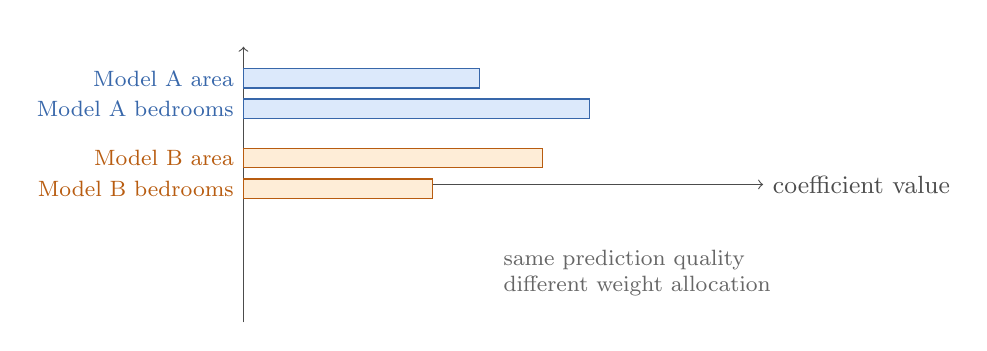
\begin{tikzpicture}[x=1cm,y=0.35cm,font=\small]
  \draw[->,black!70] (0,0) -- (6.6,0) node[right] {coefficient value};
  \draw[->,black!70] (0,-5) -- (0,5) node[above] {};
  %% Model A bars (blue)
  \fill[c3coefBg]  (0,3.5)  rectangle (3.0,4.2);
  \draw[c3coefA]   (0,3.5)  rectangle (3.0,4.2);
  \fill[c3coefBg]  (0,2.4)  rectangle (4.4,3.1);
  \draw[c3coefA]   (0,2.4)  rectangle (4.4,3.1);
  %% Model B bars (amber)
  \fill[c3coefBgAlt] (0,0.6)  rectangle (3.8,1.3);
  \draw[c3coefAlt]   (0,0.6)  rectangle (3.8,1.3);
  \fill[c3coefBgAlt] (0,-0.5) rectangle (2.4,0.2);
  \draw[c3coefAlt]   (0,-0.5) rectangle (2.4,0.2);
  %% Labels
  \node[left, font=\footnotesize, c3coefA] at (0,3.85) {Model A area};
  \node[left, font=\footnotesize, c3coefA] at (0,2.75) {Model A bedrooms};
  \node[left, font=\footnotesize, c3coefAlt] at (0,0.95) {Model B area};
  \node[left, font=\footnotesize, c3coefAlt] at (0,-0.15) {Model B bedrooms};
  \node[align=left, font=\footnotesize, black!60] at (5.0,-3.2)
    {same prediction quality\\different weight allocation};
\end{tikzpicture}%
}
\caption{Correlated features can make coefficient stories unstable. Two training runs may produce similar predictions while shifting weight between overlapping signals.}
\label{fig:correlated-feature-instability}
\end{figure}

In practice, two models trained on slightly different samples can make similar predictions while assigning noticeably different weights to correlated inputs. Prediction stays stable; interpretation does not.

\paragraph{Resampling reveals instability.} One diagnostic for coefficient fragility is to train the same model on bootstrap resamples of the training set---repeated samples drawn with replacement---and inspect how much each coefficient varies across them. A coefficient that regularly switches sign, varies wildly relative to its typical size, or whose bootstrap 95\% interval includes zero is not evidence of a stable directional effect. It may be absorbing the variance of a correlated neighbor. A stable coefficient stays in the same direction and roughly the same magnitude across resamples.

\paragraph{Adding or removing a feature changes the story.} Suppose a wage model is trained first with both years of experience and job tenure, then with tenure removed. If the experience coefficient changes substantially when tenure is dropped, that is evidence of collinearity. The original coefficient was not measuring the ``pure effect'' of experience; it was absorbing part of the tenure effect as well. This is why coefficient narratives built on a single model fit can mislead even when the model predicts well.

\begin{warningbox}
Before reporting a coefficient as evidence of a meaningful relationship, check two things: does it stay stable when correlated predictors are added or removed, and does it stay stable across resamples of the data? If either answer is no, the narrative is fragile. The model may still predict well, but the specific coefficient value should not carry the story.
\end{warningbox}

\subsection{Missing Variables Matter}

Suppose a wage model includes education but omits years of experience or industry. The education coefficient may absorb some of those missing effects. The model may still predict well, but the interpretation of that coefficient becomes less trustworthy.

\begin{example}[A Misleading Coefficient Story]
Imagine a customer-churn model in which the number of refund requests has a positive coefficient. The naive reading is that requesting refunds causes customers to leave. The more plausible explanation is that dissatisfied customers are the ones who request refunds. Predictive association is not causal explanation.
\end{example}

\begin{warningbox}
What you are usually allowed to say:
\begin{itemize}[leftmargin=*]
\item ``This feature is associated with higher predicted risk in this model.''
\item ``Holding the encoded features fixed, changing this variable moves the score in the direction of its fitted coefficient.''
\end{itemize}
What you are usually not allowed to say from the model alone:
\begin{itemize}[leftmargin=*]
\item ``This feature causes the outcome.''
\item ``Changing this feature in the world will definitely change the target by this amount.''
\end{itemize}
\end{warningbox}

These assumptions matter for inference, not for prediction alone. Linearity in the encoded features, exogeneity (zero conditional mean of the errors), independent or appropriately modeled errors, roughly constant variance, and no perfect multicollinearity are the classical conditions behind standard errors and hypothesis tests. A linear baseline can still be useful when some of those assumptions are only approximate.

\section{Prediction Is Not Intervention}

\emph{Dilemma.} The advising team's model says office-hour attendance is a strong predictor of passing the course --- the coefficient is large, the slice diagnostics are clean, and the held-out evaluation looks honest. The provost reads the report and proposes making office-hour attendance mandatory. The team must now decide what to recommend, because the question changed mid-meeting. The model predicted that students who attend office hours pass at a higher rate. The provost is asking whether \emph{forcing} the rest of the cohort to attend would raise pass rates by the same amount. Those are not the same question, and confusing them is the most expensive mistake a transparent-looking linear model invites.

Linear models tempt people into causal language because the coefficients look clean. That is where linear transparency turns dangerous if the reader stops being precise. A predictive model answers an associational question: given the observed features, what outcome should we expect? A causal question is different: what would happen if we actively changed one part of the world? Pearl's causal framework makes this distinction central by separating ordinary observation from intervention and counterfactual reasoning \citep{pearl2009}.

The distinction matters even in simple tabular problems. A model may learn that students who attend more office hours tend to earn higher grades. That makes office-hour attendance a useful predictive feature. It does \emph{not} by itself prove that forcing attendance to increase would raise grades by the same amount. Students who seek help may also be more motivated, have different schedules, or receive more support elsewhere. Those hidden differences create confounding.

\begin{warningbox}
\textbf{Observational association is not the same as causal effect.}

A fitted coefficient on observational data tells you about predictive correlation. It does not tell you what would happen if you intervened on that feature. The same coefficient could reflect a direct effect, reverse causality, hidden confounding, measurement error, or selection bias. To move from ``students who attend office hours get higher grades'' to ``providing more office hours will improve outcomes,'' you need different evidence: a randomized experiment, a quasi-experimental design, or explicit causal assumptions you have tested.
\end{warningbox}

\subsection{Confounding Changes the Story}

A \emph{confounder} is a variable that influences both the feature of interest and the outcome. When confounders are omitted or measured poorly, the fitted coefficient mixes together several stories: direct effect, indirect effect, selection effect, and historical artifact. The model can still predict well, but its coefficients are unsafe to read as intervention advice.

\begin{example}[Tutoring Is Predictive, but the Policy Claim Is Harder]
Suppose a model finds that students who sign up for tutoring are less likely to fail. Tutoring may help. Or the students who sign up early may be the same students who are more organized, more supported, or more engaged in the course. The tutoring coefficient is useful for prediction yet insufficient for the policy claim ``increasing tutoring sign-ups will reduce failure by this amount.''
\end{example}

\subsection{What Stronger Causal Language Requires}

Moving from predictive association to a causal claim raises the evidence standard. Stronger causal language usually requires a design that supports intervention reasoning: a randomized experiment, a natural experiment with defensible assumptions, or a domain model that makes the required causal assumptions explicit and testable. A fitted linear model on observational data is rarely enough on its own.

The practical rule in this book is conservative. For prediction, say ``associated with,'' ``predictive of,'' or ``raises the score when encoded features are fixed.'' Reserve words like ``causes,'' ``effect,'' or ``would improve outcomes if changed'' for settings where the causal design has actually been defended.

\section{Controlled Simplicity: Regularization}

Even linear models can overfit, especially when the feature count is large or features are noisy. Regularization addresses this by penalizing large or complex coefficient vectors. It is the chapter's answer to a practical baseline question: how do we keep the first serious model controlled without making it uselessly weak?

\begin{definition}[L2 Regularization]
L2 regularization adds a penalty proportional to the squared magnitude of the coefficients:
\[
\mathcal{L}(w,b) = \frac{1}{n}\sum_{i=1}^{n}\ell(y_i,\hat{y}_i) + \lambda \|w\|_2^2.
\]
\end{definition}

This penalty discourages extreme weights and spreads influence more smoothly across correlated features. In regression, the resulting model is called \emph{ridge regression}. The same idea applies to logistic regression for classification.

In the least-squares setting, ridge regularization also changes the optimization problem in a mathematically useful way \citep{hoerl1970}.

The theorem below uses matrix calculus fact (2) from Mathematical Bridge~I: the Hessian of $w^\top A w$ is $2A$, and $A$ being positive definite means the surface curves upward in every direction. On a first read, take the headline---``ridge gives a unique closed-form solution''---and skip the proof; it is here for readers who want to see why adding $\lambda I$ is exactly what removes the non-uniqueness of plain least squares.

\begin{theorem}[Ridge regularization gives a unique least-squares solution]
For a fixed design matrix $X$ of penalized features and any $\lambda>0$, the ridge objective
\[
J(w)=\frac{1}{n}\|y-Xw\|_2^2+\lambda\|w\|_2^2
\]
is strictly convex in $w$. Consequently it has a unique minimizer, and that minimizer satisfies
\[
(X^\top X+n\lambda I)w^\star = X^\top y.
\]
\end{theorem}

\begin{proof}
The Hessian of $J$ is
\[
\nabla^2 J(w)=\frac{2}{n}X^\top X + 2\lambda I.
\]
For any nonzero vector $v$,
\[
v^\top \nabla^2 J(w)\, v
= \frac{2}{n}\|Xv\|_2^2 + 2\lambda \|v\|_2^2 > 0
\]
because $\lambda>0$. So the Hessian is positive definite, which makes $J$ strictly convex and gives a unique minimizer. Setting the gradient to zero yields the stated linear system.
\end{proof}

\begin{definition}[L1 Regularization]
L1 regularization adds a penalty proportional to the sum of absolute coefficient values:
\[
\mathcal{L}(w,b) = \frac{1}{n}\sum_{i=1}^{n}\ell(y_i,\hat{y}_i) + \lambda \|w\|_1.
\]
\end{definition}

L1 regularization often drives some coefficients exactly to zero. That helps when we suspect only a subset of features truly matters, or when we want a sparse model that is easier to inspect.

Most implementations leave the intercept $b$ unpenalized; the regularizer is meant to control feature weights, not to drag the global baseline toward zero.

Both penalties express a preference for restrained explanations. They do not ban complexity; they require the data to justify it. That is why regularization belongs to baseline design rather than after-the-fact cleanup.

The geometry gives a useful picture. The L2 penalty has round contours, so optimization tends to shrink many weights smoothly. The L1 penalty has diamond-shaped contours with corners on the axes, so solutions are more likely to land exactly on an axis, which is why zeros appear naturally.

\begin{figure}[t]
\centering
\definecolor{c3l2Blue}{RGB}{56,103,170}
\definecolor{c3l1Amber}{RGB}{184,92,16}
\definecolor{c3l2BgLight}{RGB}{220,233,251}
\definecolor{c3l1BgLight}{RGB}{254,237,215}
\resizebox{\linewidth}{!}{%
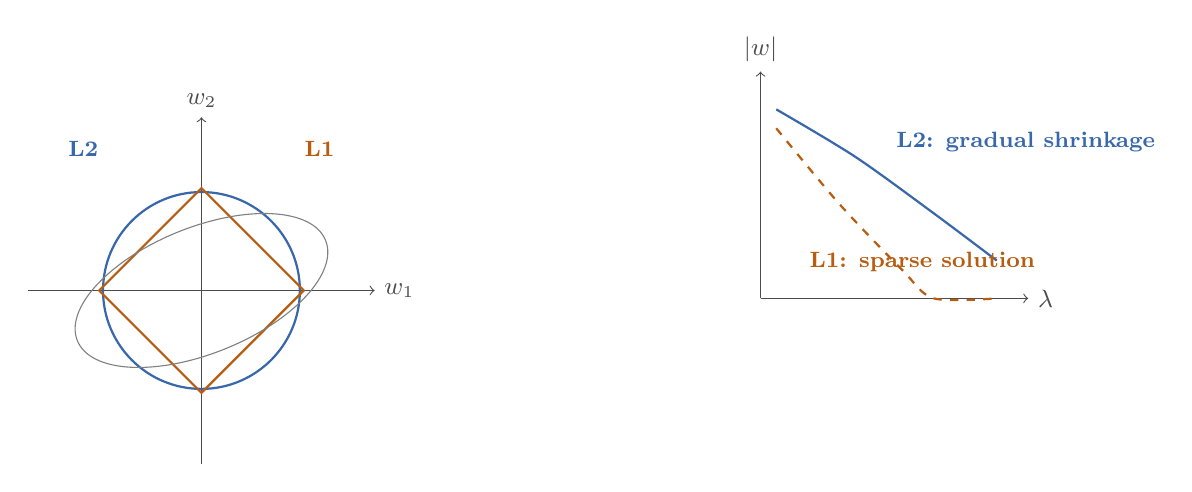
\begin{tikzpicture}[font=\small]
%% Panel A: constraint geometry
\begin{scope}
  \draw[->,black!70] (-2.2,0) -- (2.2,0) node[right] {$w_1$};
  \draw[->,black!70] (0,-2.2) -- (0,2.2) node[above] {$w_2$};
  %% L2 circle (blue)
  \draw[c3l2Blue,thick] (0,0) circle (1.25);
  %% L1 diamond (amber)
  \draw[c3l1Amber,thick] (-1.3,0) -- (0,1.3) -- (1.3,0) -- (0,-1.3) -- cycle;
  %% Loss ellipse (gray)
  \draw[black!50,rotate around={22:(0,0)}] (0,0) ellipse (1.7 and 0.8);
  \node[c3l2Blue,  font=\footnotesize\bfseries] at (-1.5,1.8) {L2};
  \node[c3l1Amber, font=\footnotesize\bfseries] at (1.5,1.8)  {L1};
\end{scope}
%% Panel B: shrinkage paths
\begin{scope}[xshift=7.1cm,yshift=-0.1cm,x=1.0cm,y=1.2cm]
  \draw[->,black!70] (0,0) -- (3.4,0) node[right] {$\lambda$};
  \draw[->,black!70] (0,0) -- (0,2.4) node[above] {$|w|$};
  %% L2: gradual smooth shrinkage
  \draw[c3l2Blue,thick] plot[smooth] coordinates {(0.2,2.0)(1.2,1.5)(2.2,0.9)(3.0,0.4)};
  %% L1: drops to zero
  \draw[c3l1Amber,thick,dashed] plot[smooth] coordinates {(0.2,1.8)(1.0,1.0)(1.8,0.3)(2.2,0.0)(3.0,0.0)};
  \node[c3l2Blue,  anchor=west, font=\footnotesize\bfseries] at (1.6,1.65) {L2: gradual shrinkage};
  \node[c3l1Amber, anchor=west, font=\footnotesize\bfseries] at (0.5,0.38) {L1: sparse solution};
\end{scope}
\end{tikzpicture}%
}
\caption{L2 regularization prefers smaller coefficients smoothly. L1 regularization can drive some coefficients all the way to zero. Validation, not taste, should decide how much regularization is appropriate.}
\label{fig:l1-l2-regularization}
\end{figure}

Regularization strength $\lambda$ is not an aesthetic preference. It is a model-selection choice and should be chosen by validation performance. This is also why standardization matters more once regularization is active: if one feature sits on a much larger scale than another, the penalty no longer treats them comparably.

Suppose validation accuracy for ridge-logistic baselines is
\[
\begin{array}{c|ccc}
\lambda & 0.001 & 0.1 & 10 \\
\hline
\text{train accuracy} & 0.96 & 0.91 & 0.78 \\
\text{validation accuracy} & 0.82 & 0.88 & 0.76
\end{array}
\]
The smallest penalty fits training best but generalizes worse; the largest underfits both training and validation. The middle value is the defensible baseline choice because validation evidence, not the prettiest coefficient story, selected it.

\begin{codeexample}[caption={From scratch: L2 gradient versus an L1 subgradient sketch}]
# Both penalties are added to the data-loss gradient before each weight update.
# lam is the regularization strength; weights is the current weight vector.

# L2 penalty gradient: proportional to the weight itself (smooth shrinkage)
l2_penalty_gradient = [2 * lam * w for w in weights]

# L1 penalty subgradient: sign away from zero; choose 0 at the kink for this sketch
def sign(v):
    return 1 if v > 0 else (-1 if v < 0 else 0)

l1_penalty_subgradient = [lam * sign(w) for w in weights]

# Combined update step (choose one penalty):
# weights[j] -= learning_rate * (data_gradient[j] + l2_penalty_gradient[j])
# weights[j] -= learning_rate * (data_gradient[j] + l1_penalty_subgradient[j])
\end{codeexample}

The L2 penalty nudges every weight toward zero by an amount proportional to its current value. Large weights shrink faster than small ones, and under ordinary gradient-style updates they are driven toward zero smoothly rather than snapped exactly to zero by the penalty alone. The L1 penalty moves every non-zero weight by the same fixed step regardless of magnitude, which is why it can drive weights all the way to zero and produce sparse models. Because the absolute-value penalty is not differentiable at zero, the code above is intentionally a subgradient-style sketch rather than a literal everywhere-differentiable gradient update.

\section{The Bias--Variance Decomposition}
\label{sec:bias-variance}

\emph{Dilemma.} The team retrains the advising model after a regularization sweep. The lightly regularized model has near-zero training error but its predictions on next semester's hold-out cohort jump around wildly --- a single new student profile sometimes flips the recommendation. The heavily regularized model is stable across hold-out cohorts but predicts every student to the same middle of the score range. The team is told to ``just pick the one with the lowest validation error,'' and the recommendation works. But it works without naming the two different failures the two models embody, and the team has no language for what regularization actually bought. That language is the bias--variance decomposition.

Regularization was introduced as ``controlled simplicity,'' and the practical intuition was clear: a smaller model overfits less. The formal version of that intuition is the bias--variance decomposition, which says exactly what generalization error is made of and what regularization is trading.

\subsection{Setting Up the Question}

A trained model $\hat{f}_D$ depends on the particular training set $D$ it saw. Drawing a different training set from the same distribution gives a different fitted model. We do not usually think about this dependence explicitly, because we work with one $D$ at a time. The decomposition makes it explicit.

Fix an input $x_0$ and imagine the thought experiment: draw many training sets $D_1, D_2, \ldots$ from the same data distribution, train a model on each, and look at the predictions $\hat{f}_{D_1}(x_0), \hat{f}_{D_2}(x_0), \ldots$ at the same query point. The randomness in these predictions has two sources: the noise that turned the true target into an observed label, and the sample-to-sample variation in which $D$ was drawn.

\begin{quote}\itshape
Generalization error is not one quantity. It is a sum of three things: how wrong the model class is on average, how wide its predictions vary across training sets, and how noisy the world is.
\end{quote}

\subsection{The Decomposition}

Assume a target generated by an unknown function plus zero-mean noise:
\[
y \;=\; f(x) + \varepsilon, \qquad \mathbb{E}[\varepsilon]=0, \qquad \mathrm{Var}(\varepsilon)=\sigma^2.
\]
At a query point $x_0$, the expected squared error of a learned model $\hat{f}_D$, averaging over both the noise $\varepsilon$ and the training set $D$, decomposes as
\[
\mathbb{E}_{D,\varepsilon}\!\left[(y - \hat{f}_D(x_0))^2\right]
\;=\;
\underbrace{\bigl(f(x_0) - \mathbb{E}_D[\hat{f}_D(x_0)]\bigr)^2}_{\text{bias}^2}
\;+\;
\underbrace{\mathrm{Var}_D\bigl(\hat{f}_D(x_0)\bigr)}_{\text{variance}}
\;+\;
\underbrace{\sigma^2}_{\text{noise}}.
\]
The three terms have separate meanings. Bias is systematic error: how far the average prediction across training sets is from the truth. Variance is the spread of predictions across training sets. Noise is the irreducible part---the floor below which no model can go, no matter how rich or how regularized.

\textbf{Where the decomposition comes from (skip on a first pass).} Let $\bar{f}(x_0) = \mathbb{E}_D[\hat{f}_D(x_0)]$ denote the expected prediction at $x_0$, averaging over training sets. Add and subtract $\bar{f}(x_0)$ and $f(x_0)$ inside the squared error:
\[
y - \hat{f}_D(x_0) \;=\; \underbrace{(y - f(x_0))}_{\varepsilon} \;+\; \underbrace{(f(x_0) - \bar{f}(x_0))}_{\text{bias}} \;+\; \underbrace{(\bar{f}(x_0) - \hat{f}_D(x_0))}_{\text{centered model deviation}}.
\]
Square this expression. The three cross-terms vanish in expectation: $\varepsilon$ has mean zero and is independent of $D$; the centered model deviation $\bar{f}(x_0) - \hat{f}_D(x_0)$ has mean zero across $D$; and the bias term $f(x_0) - \bar{f}(x_0)$ is a constant under both expectations. What is left is the sum of three squared terms, which is exactly the decomposition above. The argument requires only the independence of $\varepsilon$ from $D$ and zero-mean noise; it makes no assumption about the model class. A first-pass reader can take the three-term formula as a fact about expected squared error; the derivation is for readers who want to see why the cross-terms vanish.

\subsection{Reading the Decomposition}

The three terms tell different stories.

\textbf{Bias} measures how restrictive the model class is. If $f$ is genuinely nonlinear and we fit it with a straight line, the line's average prediction across training sets cannot match the truth---the bias is structural, not a training failure. A richer model class has more flexibility to bring its average closer to $f$, which reduces bias.

\textbf{Variance} measures how much the fitted model depends on the particular training set. A model class flexible enough to fit any small wiggle of the training data will produce very different fits on different $D$'s, even when the underlying $f$ has not changed. Variance grows with model complexity and shrinks when there is more data or more constraint on the parameters.

\textbf{Noise} is the irreducible target uncertainty. The labels themselves vary for reasons no feature available to the model captures. The decomposition makes it visible that no amount of model engineering can reduce this floor.

The headline tradeoff: increasing model complexity typically reduces bias and increases variance, while decreasing model complexity does the reverse. Generalization error is minimized somewhere in the middle.

\begin{figure}[t]
\centering
\resizebox{0.9\linewidth}{!}{%
\begin{tikzpicture}[font=\small, x=1.1cm, y=1.0cm]
% Axes
\draw[->] (0,0) -- (8.4,0) node[below right, font=\footnotesize] {model complexity};
\draw[->] (0,0) -- (0,4.4) node[above left, font=\footnotesize] {expected error};
% Bias squared: decreasing curve
\draw[boxBlue, line width=1.2pt, smooth, domain=0.3:8]
  plot (\x, {2.8*exp(-0.55*\x) + 0.05});
\node[boxBlue, anchor=west, font=\footnotesize] at (6.0,0.45) {bias$^2$};
% Variance: increasing curve
\draw[boxAmber, line width=1.2pt, smooth, domain=0.3:8]
  plot (\x, {0.10*exp(0.40*\x)});
\node[boxAmber, anchor=west, font=\footnotesize] at (6.6,3.8) {variance};
% Total error: sum of bias^2 + variance (+ noise constant)
\draw[boxGreen, line width=1.5pt, smooth, domain=0.3:8]
  plot (\x, {2.8*exp(-0.55*\x) + 0.05 + 0.10*exp(0.40*\x) + 0.4});
\node[boxGreen, anchor=west, font=\footnotesize] at (6.0,3.05) {total};
% Noise floor (dashed)
\draw[dashed, gray] (0,0.4) -- (8.0,0.4);
\node[gray, anchor=west, font=\footnotesize] at (5.0,0.20) {noise floor $\sigma^2$};
% Optimum marker
\draw[dotted, gray] (3.0,0) -- (3.0,1.45);
\node[font=\footnotesize, anchor=north] at (3.0,0) {optimum};
\end{tikzpicture}%
}
\caption{The classic bias--variance picture. Bias shrinks as the model class grows. Variance grows as the model class grows. Their sum (plus a noise floor) has a minimum at some intermediate complexity, which is what cross-validation and regularization try to find.}
\label{fig:bias-variance}
\end{figure}

\subsection{Watching the Tradeoff in Code}

The cleanest way to see the decomposition is to simulate the thought experiment. Draw many training sets, fit a polynomial regression at a range of degrees, and measure bias$^2$ and variance directly at a held-out query point.

\begin{codeexample}
import numpy as np

def true_f(x):
    return np.sin(2 * np.pi * x)             # smooth target

def make_dataset(n, sigma, rng):
    x = rng.uniform(0, 1, size=n)
    y = true_f(x) + sigma * rng.standard_normal(size=n)
    return x, y

def fit_poly(x, y, degree):
    # Closed-form least squares on a polynomial design matrix.
    Phi = np.vander(x, N=degree + 1, increasing=True)
    w, *_ = np.linalg.lstsq(Phi, y, rcond=None)
    return w

def predict(w, x):
    Phi = np.vander(x, N=len(w), increasing=True)
    return Phi @ w

# Monte-Carlo estimate of bias^2 and variance at a grid of query points.
rng         = np.random.default_rng(0)
n_train     = 30
sigma       = 0.30
n_runs      = 500
x_query     = np.linspace(0, 1, 50)
f_query     = true_f(x_query)

for degree in [1, 3, 9, 15]:
    preds = np.zeros((n_runs, len(x_query)))
    for r in range(n_runs):
        x, y = make_dataset(n_train, sigma, rng)
        w    = fit_poly(x, y, degree)
        preds[r] = predict(w, x_query)
    mean_pred = preds.mean(axis=0)
    bias2     = ((mean_pred - f_query) ** 2).mean()
    variance  = preds.var(axis=0).mean()
    print(f"degree={degree:2d}   "
          f"bias^2={bias2:.3f}   variance={variance:.3f}   "
          f"sum={bias2 + variance:.3f}")
# degree= 1   bias^2=0.250   variance=0.012   sum=0.262   <- underfit
# degree= 3   bias^2=0.009   variance=0.024   sum=0.033
# degree= 9   bias^2=0.002   variance=0.103   sum=0.105
# degree=15   bias^2=0.001   variance=0.380   sum=0.381   <- overfit
\end{codeexample}

The numbers do exactly what the theory predicts. The degree-$1$ fit cannot reach a sine wave: its bias is large and its variance is small. The degree-$15$ fit can in principle express the sine wave perfectly, but with only thirty training points it fits the noise, so its bias is small and its variance is huge. Degree $3$ is the sweet spot for this setup---small enough to keep variance contained, large enough to capture the curvature. A second run with a larger $n_{\text{train}}$ would push the optimum higher, because variance shrinks with more data while bias does not.

\subsection{Ridge as a Variance Reducer}

The decomposition gives the formal justification for regularization. Ridge regression shrinks coefficients toward zero, which lowers variance but introduces bias. With weight decay $\lambda > 0$, the closed-form solution becomes
\[
\hat{w}_{\lambda} \;=\; (X^\top X + \lambda I)^{-1} X^\top y.
\]

\textbf{Ridge bias and variance, in closed form (Extension).} For a linear model with true coefficients $w^\star$, the ridge estimator has bias $\mathbb{E}[\hat{w}_\lambda] - w^\star = -\lambda (X^\top X + \lambda I)^{-1} w^\star$, which vanishes at $\lambda = 0$ and grows monotonically with $\lambda$. Its variance is proportional to $(X^\top X + \lambda I)^{-1} X^\top X (X^\top X + \lambda I)^{-1}\sigma^2$, which is largest at $\lambda = 0$ and shrinks toward zero as $\lambda$ grows. The trade is explicit: $\lambda$ buys lower variance at the cost of higher bias, and cross-validation chooses the $\lambda$ that minimizes the sum. A first-pass reader can stop at ``ridge trades a little bias for a lot of variance''; the closed-form formulas above are for readers who want to see exactly how $\lambda$ rescales each direction in parameter space.

The decomposition is a thinking tool, not a measurement tool. In practice, only the sum of bias$^2$ and variance is observed---as held-out error---and they are estimated, not isolated, except in simulations like the one above. Use the decomposition to reason about why a model is failing (high bias \emph{vs.} high variance) and what to change (richer model class, more data, more regularization), but do not expect to read bias and variance off a single experiment.

\begin{decisionbox}
\textbf{When the error is too high, ask which term is at fault.} If train and test errors are both high and close together, suspect bias---the model class cannot represent the target. Add features, switch to a more flexible family, or remove regularization. If train error is low but test error is high, suspect variance---the model has memorized the particular training set. Add data, add regularization, or move to a simpler model. The bias--variance decomposition is the formal version of this diagnostic.
\end{decisionbox}

\section{Sparse Linear Models Stay Strong in Text and Tabular Work}

A persistent misconception is that linear models are only a warm-up before the real work with deep models begins. In several important problem families, sparse linear models remain genuinely strong baselines, not compromises.

\textbf{Text classification.} A bag-of-words or TF--IDF representation with logistic regression often reaches accuracy on news topic classification, spam filtering, or sentiment classification within a few percentage points of deep models, at a fraction of the cost. The reason is straightforward: in text classification, the vocabulary already exposes the relevant signal. A word like ``inheritance'' is informative about legal topics; a word like ``free'' is informative about spam. A linear model on a well-engineered bag-of-words finds those associations efficiently.

\textbf{High-dimensional tabular prediction.} In fraud detection, credit scoring, and clinical risk modeling, datasets often have hundreds or thousands of engineered features over millions of examples. Many features are individually informative, and their combination is largely additive. A regularized linear model handles this well. The L1 penalty can yield a sparse set of nonzero coefficients, easing inspection---though selected features still need stability and domain checks before being treated as genuinely informative or interpretable. Tree ensembles often win eventually, but rarely by a margin that justifies a tenfold increase in compute during initial prototyping.

\begin{example}[Linear Baseline on a Text Task]
For a news topic classifier over four categories, logistic regression with TF--IDF features might reach $93\%$ accuracy and a fine-tuned transformer $96\%$. That three-point gap may matter for a production system, but it does not mean the linear baseline was uninformative. It established that the task is solvable, showed which categories confuse the model, and provided the reference point against which the expensive model must justify its cost.
\end{example}

\textbf{Baseline ladder in text and tabular work.} Before training any deep model, ask whether a regularized logistic or linear regression on engineered features already works well. If it does, the deep model must offer either a meaningful accuracy gain on the evaluation set or a well-justified argument for why it will perform better in production. Neither argument is hard to make, but both should be made explicitly.

The broader point is that linear models expose the relationship between representation and prediction transparently. When they succeed, they reveal something about the problem's structure: it was largely additive in the feature space you chose. When they fail by a large margin, they reveal something even more useful: the problem contains interactions, local geometry, or sequential structure that the feature set could not capture. Either result is informative. The deep model that follows should be chosen in response to that specific structural diagnosis.

\section{Failure Diagnosis, Not Method Shopping}

No model family is universal. Linear models struggle when the decision boundary or regression surface cannot be captured by a weighted sum of the available features. Images, audio, and raw language sequences often contain local, hierarchical, or contextual structure that a linear score cannot exploit directly unless something else has already encoded it.

They also struggle when interactions are essential but omitted. If one feature's effect depends strongly on another and that interaction is not encoded explicitly, a linear model can be systematically wrong even when each feature is individually informative.

That is the right way to think about moving beyond linear models. Do not abandon them because a richer family is fashionable. Abandon them only when the problem or the evidence shows that the needed structure cannot be captured in the current representation.

\begin{figure}[t]
\centering
\definecolor{c3cls1}{RGB}{56,103,170}
\definecolor{c3cls2}{RGB}{184,92,16}
\definecolor{c3sepLine}{RGB}{26,112,64}
\resizebox{\linewidth}{!}{%
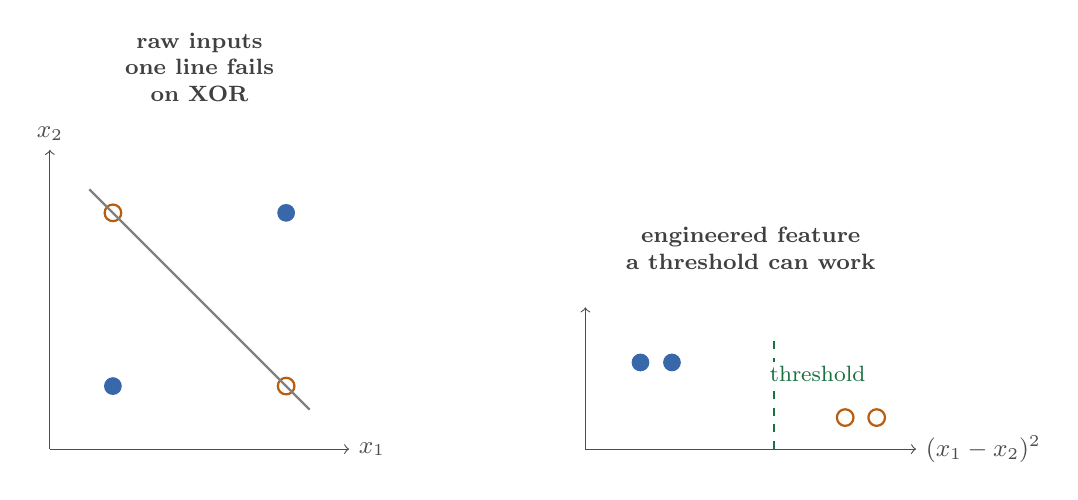
\begin{tikzpicture}[
  font=\small,
  paneltitle/.style={
    font=\footnotesize\bfseries,
    align=center,
    fill=white,
    inner sep=2pt,
    rounded corners=2pt,
    text=black!75
  }
]
%% Panel A: XOR – single line fails
\begin{scope}
  \draw[->,black!70] (0,0) -- (3.8,0) node[right] {$x_1$};
  \draw[->,black!70] (0,0) -- (0,3.8) node[above] {$x_2$};
  %% Class 1 (blue filled)
  \filldraw[fill=c3cls1,draw=c3cls1] (0.8,0.8) circle (3pt);
  \filldraw[fill=c3cls1,draw=c3cls1] (3.0,3.0) circle (3pt);
  %% Class 2 (amber open)
  \draw[c3cls2,thick] (0.8,3.0) circle (3pt);
  \draw[c3cls2,thick] (3.0,0.8) circle (3pt);
  %% A line that doesn't separate them
  \draw[black!50,thick] (0.5,3.3) -- (3.3,0.5);
  \node[paneltitle, text width=3.2cm] at (1.9,4.85)
    {raw inputs\\one line fails on XOR};
\end{scope}
%% Panel B: engineered feature separates
\begin{scope}[xshift=6.8cm]
  \draw[->,black!70] (0,0) -- (4.2,0) node[right] {$(x_1 - x_2)^2$};
  \draw[->,black!70] (0,0) -- (0,1.8);
  \filldraw[fill=c3cls1,draw=c3cls1] (0.7,1.1) circle (3pt);
  \filldraw[fill=c3cls1,draw=c3cls1] (1.1,1.1) circle (3pt);
  \draw[c3cls2,thick] (3.3,0.4) circle (3pt);
  \draw[c3cls2,thick] (3.7,0.4) circle (3pt);
  \draw[c3sepLine,thick,dashed] (2.4,0) -- (2.4,1.4);
  \node[c3sepLine, font=\footnotesize, fill=white, inner sep=1.5pt] at (2.95,0.95) {threshold};
  \node[paneltitle, text width=3.6cm] at (2.1,2.55)
    {engineered feature\\a threshold can work};
\end{scope}
\end{tikzpicture}%
}
\caption{Failure should be diagnosed structurally. Sometimes one weighted sum on raw inputs is not enough, but a better feature map can rescue the linear model. Other times a different model family is needed.}
\label{fig:linear-model-failure}
\end{figure}

The diagnostic questions are often more useful than the answer:
\begin{itemize}[leftmargin=*]
\item If interactions are missing, perhaps trees or engineered interaction features matter.
\item If a plausible feature space needs a more robust separator, perhaps margin-based methods matter.
\item If sparse class-conditional patterns matter, perhaps a probabilistic baseline such as Naive Bayes matters.
\item If local neighborhoods matter, perhaps nearest-neighbor ideas matter.
\item If unlabeled structure matters, clustering or dimensionality reduction may matter.
\item If raw images or sequences matter, learned representations may matter later.
\end{itemize}

That is why the next chapter is the natural move. It does not replace linear thinking. It asks a sharper structural question: is the missing piece mainly conditional thresholds and interactions, margin structure, class-conditional probabilistic structure, local similarity, or unlabeled organization? The weighted-sum baseline makes that diagnosis possible.

\section{Chapter Artifact: A First Baseline Design Sheet}

By the end of this chapter, the reader should be able to write down the first defensible baseline before trying more expressive methods. The goal is not to freeze creativity but to make the first modeling move explicit enough that later changes become justified rather than impulsive. The framing memo named the decision context, the metric worksheet named good behavior, and the evaluation plan protected the claim. This sheet names the first serious model that deserves to make that claim. It is where the representation audit and the baseline ladder turn into one written modeling commitment.

\begin{table}[t]
\centering
\small
\setlength{\tabcolsep}{4pt}
\begin{tabular}{p{3.23cm}p{7.0cm}}
\toprule
Design field & What must be stated clearly \\
\midrule
Seven-question focus & Questions 4, 5, and 6: choose the representation, justify the first serious baseline, and state what evidence would show that linearity is no longer enough \\
Task and target type & Regression or classification, and what the model is being asked to predict \\
Raw input & What the original data looks like before encoding \\
Feature map & Which engineered or encoded features the weighted sum will actually see \\
Baseline model & Linear regression, logistic regression, or another linear baseline appropriate to the target \\
Regularization choice to validate & Which penalty strengths or types will be compared using validation data \\
Interpretation boundary & What coefficients would and would not justify saying about the world \\
Failure pattern to watch for & What kind of error would indicate that one weighted sum is missing important structure \\
Next structural hypothesis & What broader model family would be justified if the baseline fails for the named reason \\
\bottomrule
\end{tabular}
\caption{If this sheet cannot be written, the first baseline is usually underdesigned rather than underpowered.}
\label{tab:baseline-design-sheet}
\end{table}

\textbf{Baseline design sheet.} Before training the first serious model, write down the representation, baseline family, regularization choices, interpretation boundary, and what kind of failure would justify moving beyond linearity.

\begin{example}[Filled Baseline Design Sheet]
For early student-support prediction, the raw input might be course activity logs, attendance, and the first assignment timeline. The feature map could expose missed-deadline count, recent platform inactivity, quiz completion rate, and---if recorded before the model decision point---whether the student had already triggered an earlier administrative flag. The first baseline would be logistic regression with validation over a small range of regularization strengths. The interpretation boundary would state that coefficients describe the baseline's evidence pattern, not causal claims about why a student disengages. The named failure pattern might be weak performance on students whose problems appear only through timing or sequence order, which would justify moving next to a sequential model rather than jumping blindly to a more complex classifier.
\end{example}

\section{Common Mistakes with Linear Models}

The common mistakes with linear models are predictable. Teams treat feature engineering as mechanical even though representation is already part of the model. They overread coefficients as if fitted associations were causal structure. They encode nominal categories as fake numeric order. They ignore missingness as a possible signal. They skip standardization even when regularization makes scale consequential. And they jump past the linear baseline before learning what it can already explain. Most of these errors are not failures of algebra; they are failures of interpretation.

\section{Looking Ahead}

This chapter showed that representation is already part of the model. The next chapter studies what kind of structure is missing when one global weighted sum is not enough: conditional thresholds and interactions, margin structure, class-conditional probabilistic structure, local similarity, or unlabeled organization.

\section*{Chapter Summary}

This chapter argued that linear modeling is first a representation test and only second a fitting procedure. Once raw inputs are encoded into features, linear regression and logistic regression become two versions of the same weighted-sum pipeline, differing mainly in output transform and target type. The chapter also showed why coefficient reading requires restraint: scale, collinearity, omitted variables, and the distinction between prediction and intervention each shape what a coefficient can honestly mean. Regularization then turns a simple model into a controlled baseline, and the real value of that baseline is diagnostic. If it succeeds, the task may already be largely additive in the chosen feature space. If it fails, the pattern of failure shows what structure is missing.

\begin{table}[ht]
\centering
\small
\caption{Where Chapter~\ref{ch:linear-models} ideas return.}
\label{tab:ch3-forward}
\begin{tabular}{@{}L{3.15cm}L{6.65cm}@{}}
\toprule
\textbf{Topic} & \textbf{Returns in} \\
\midrule
Representation \& feature maps & Chapter~\ref{ch:structure-beyond-linearity} (nonlinear structure; when hand-crafted features are not enough) \\
Feature interactions \& basis expansion & Chapter~\ref{ch:optimization-neural-networks} (learned feature combinations; neural networks as learned basis) \\
Linear separability \& decision boundaries & Chapter~\ref{ch:optimization-neural-networks} (activation functions create piecewise-linear boundaries) \\
Coefficient interpretation & Chapter~\ref{ch:experiments-claims} (claims, ablation, model diagnostics, causal reasoning) \\
Scale sensitivity \& standardization & Chapters~\ref{ch:optimization-neural-networks} and~\ref{ch:representation-foundation-models} (batch normalization, learned scaling) \\
Regularization \& overfitting control & Chapters~\ref{ch:optimization-neural-networks} and~\ref{ch:reliability} (weight decay, generalization, robustness) \\
Baseline design sheet & Chapters~\ref{ch:structure-beyond-linearity} and~\ref{ch:models-systems} (structural diagnosis, readiness brief) \\
\bottomrule
\end{tabular}
\end{table}

\begin{studyquestions}
\item Why is ``can one weighted sum already solve the task?'' a better opening question than ``which regression formula comes first?'' 
\item In what sense is representation already part of the model?
\item Why can a model be linear even when the relationship between the raw input and target is not?
\item Why can correlated features make coefficient interpretation unstable even when prediction stays good?
\item Why is a predictive association not the same as evidence for an intervention?
\item What kind of failure would justify leaving a linear baseline for a different model family?
\end{studyquestions}

\begin{exercises}
\item \exercisetag{Concept}{Core}One-hot encoding drill: encode the categorical variable \emph{browser} with possible values \{Chrome, Firefox, Safari\} for an example in which the browser is Safari.
\item \exercisetag{Concept}{Core}Sparse bag-of-words drill: suppose the vocabulary is \{free, cash, meeting, project\} and the email text is ``free project cash.'' Write the bag-of-words vector and compute its dot product with weights $[1.2, 0.8, -0.5, -0.3]$.
\item \exercisetag{Concept}{Core}Representation audit: for a task of your choice, state the raw input, the encoded representation, one thing the representation loses, and one assumption it inserts.
\item \exercisetag{Concept}{Core}Logit-to-probability drill: convert logits $-1.5$, $0$, and $1.5$ into probabilities using the sigmoid function.
\item \exercisetag{Concept}{Intermediate}Score-to-boundary drill: explain why a logistic-regression threshold of $0.5$ is equivalent to testing whether the linear score is nonnegative. Then, for $w=[2,-1]$ and $b=-0.5$, write the boundary equation.
\item \exercisetag{Design}{Intermediate}Which feature map makes this relation more linear? A target grows slowly for small $x$ and much faster for large $x$. Suggest one transformed feature set that could help a linear model fit that pattern better.
\item \exercisetag{Concept}{Intermediate}Same prediction, different coefficients: explain how two models could make similar predictions while assigning different weights to area and bedrooms in a housing model.
\item \exercisetag{Concept}{Intermediate}L1 or L2? Give one situation where sparse feature selection is especially useful and one situation where smooth shrinkage across correlated features is more appropriate.
\item \exercisetag{Concept}{Intermediate}A model finds that students who attend more office hours tend to earn higher grades. Write one predictive interpretation and one intervention claim that the model does \emph{not} justify by itself.
\item \exercisetag{Design}{Intermediate}Use a public tabular task such as sports-shot prediction and propose a first linear baseline with 4--6 features, a target type, and one failure pattern you would watch for.
\item \exercisetag{Design}{Intermediate}Write language-neutral pseudocode that takes a feature vector, weights, and a bias, then returns the logistic score, probability, and thresholded label.
\item \exercisetag{Design}{Intermediate}Use Table~\ref{tab:baseline-design-sheet} to write a one-page baseline design sheet for either spam filtering, student support, or another application of your choice. If you are carrying one case through the book, inherit the same task from the earlier framing, metric, and evaluation artifacts, then end by naming the next structural hypothesis you would test if the linear baseline fails.
\item \exercisetag{Implementation}{Core}Implement linear regression two ways on a synthetic three-feature dataset of $n=200$ points. Generate $X \in \mathbb{R}^{200\times 3}$ from a standard normal, set $y = X w^\star + 0.1\,\varepsilon$ for some known $w^\star$ and Gaussian noise $\varepsilon$, then (a) compute the closed-form OLS solution $\hat w = (X^\top X)^{-1} X^\top y$, and (b) recover the same $\hat w$ by running 1{,}000 gradient-descent steps on the squared-error loss with a learning rate you choose. Plot the loss-vs.-iteration curve and report $\|\hat w_{\text{GD}} - \hat w_{\text{OLS}}\|_2$. Confirm that both estimates also approximately recover $w^\star$.
\item \exercisetag{Implementation}{Intermediate}Extend the previous exercise to logistic regression on the same three features but binarized labels $y_i = \mathbb{1}\{X_i w^\star + \varepsilon_i > 0\}$. Implement the negative log-likelihood, its gradient, and 500 gradient-descent steps. Plot the decision boundary on a 2D slice of feature space, then change the learning rate by a factor of 10 in each direction and report which loss curves diverge, oscillate, or simply slow down.
\item \exercisetag{Proof}{Advanced}Show that the logistic negative log-likelihood is convex in $w$. Write the loss for a single example $(x_i, y_i)$ as $\ell_i(w) = -y_i \log \sigma(x_i^\top w) - (1 - y_i)\log(1 - \sigma(x_i^\top w))$. Compute $\nabla_w \ell_i$ and $\nabla_w^2 \ell_i$ explicitly using $\sigma'(z) = \sigma(z)(1 - \sigma(z))$. Show that the per-example Hessian is $\sigma(x_i^\top w)(1 - \sigma(x_i^\top w))\, x_i x_i^\top$, which is positive semi-definite for any $x_i$. Conclude that the full empirical NLL --- a sum of per-example terms --- is also convex. State explicitly when the loss is \emph{strictly} convex versus only convex.
\item \exercisetag{Proof}{Advanced}Derive the closed-form ridge bias and variance. With ridge estimator $\hat w_\lambda = (X^\top X + \lambda I)^{-1} X^\top y$ under the linear model $y = X w^\star + \varepsilon$ with $\mathbb{E}[\varepsilon] = 0$ and $\mathrm{Cov}(\varepsilon) = \sigma^2 I$, show that (a) $\mathbb{E}[\hat w_\lambda] = (X^\top X + \lambda I)^{-1} X^\top X w^\star$, (b) the bias is $\mathbb{E}[\hat w_\lambda] - w^\star = -\lambda(X^\top X + \lambda I)^{-1} w^\star$, and (c) the variance is $\sigma^2 (X^\top X + \lambda I)^{-1} X^\top X (X^\top X + \lambda I)^{-1}$. Confirm that both quantities vanish at $\lambda = 0$ for the variance and at $\lambda = 0$ for the bias respectively, and that bias grows monotonically with $\lambda$ while variance shrinks monotonically.
\end{exercises}

\begin{challengeexercises}
\item \exercisetag{Calculation}{Intermediate}A logistic model has coefficients $w = [1.2, -0.8, 0.5]$, bias $b=-0.4$, and feature vector $x=[2,1,3]$. Compute the linear score, the predicted probability, and the final predicted label if the threshold is $0.5$.
\item \exercisetag{Design}{Advanced}Propose a nonlinear real-world relationship that can still be modeled by a linear model after feature engineering. State the transformed features explicitly and explain why the model remains linear in the parameters.
\item \exercisetag{Design}{Advanced}Construct a small binary-classification task in which one weighted sum on the raw inputs fails, but one additional transformed feature rescues the linear model. State the transformed feature and explain why the rescue works.
\item \exercisetag{Concept}{Advanced}Give an example in which a coefficient is highly interpretable for prediction but misleading for causal inference. Explain what additional assumptions or data would be needed before making a causal claim.
\item \exercisetag{Diagnosis}{Advanced}Take one failed linear baseline result from your own experience or invent one. Diagnose the failure structurally: what missing interaction, locality, sequence effect, or learned representation would justify the next modeling step?
\end{challengeexercises}
